\section{Third-order correlation analysis}

In this section, we analyse the resistance of the implementation against third order side-channel analysis based on the linear correlation coefficient (CPA). For this study, we will target the Sbox output value and consider a Hamming weight ($HW$) univariate leakage model.

In the remainder of this section, we will use:
\begin{itemize}

\item the centered product combination function $\mathcal{C}(x,y,z) = (x-\overline{x})(y-\overline{y})(z-\bar{z})$ to preprocess the traces, where $\overline{x}$ (resp. $\overline{y}$, $\bar{z}$) stands for the mean value of $x$ (resp. $y$, $z$), computed on all traces in our campaign; 

\item the corresponding function $f_{HW}(z) = \sum_{m,m'} (HW(m'\times z \oplus m) -\\ \overline{HW(m'\times z\oplus m)})(HW(m)-\overline{HW(m)})(HW(m')-\overline{HW(m')})$ to compute the predictions, where $\overline{HW(m)}$ (resp $\overline{HW(m'\times z \oplus m)}$, $\overline{HW(m')}$) stands for the mean value of $HW(m)$ (resp. $HW(m' \times z\oplus m)$, $HW(m')$) computed on all possible values of $m,m'$\footnote{Note that all possible values for $m$ are in $[0,255]$, while all possible values for $m'$ are in $[1,255]$.}.
\end{itemize}

As in our first-order and second-order correlation analyses, we will split this study in two parts. The first part will consider priviledged knowledge on the mask values. The second part will not consider this knowledge.

\subsection{Priviledged knowledge}
We first study the setting where the attacker knows the random masks used to compute the permutation. 

In order to characterize the effectiveness of a CPA against this implemenation, we use the random masks to recompute the permutation $Sh(i)$ for each byte index $i$.

\subsubsection{Raw Sbox output}
We target the value $Z_{\hat{k}}[i]$ for any hypothesis $k$.
The attack does not succeed using the $100.000$ traces.
%/media/nas/projects/ASCAD_CW/ASCAD_ChipWhisperer/ARM/traces/attack_results_3O_without_flaw_fixed_100k.h5
Figure~\ref{fig:CPA3O_trickedZ1} illustrates the results using $100000$ traces.
\begin{figure}[H]
	\centering 
	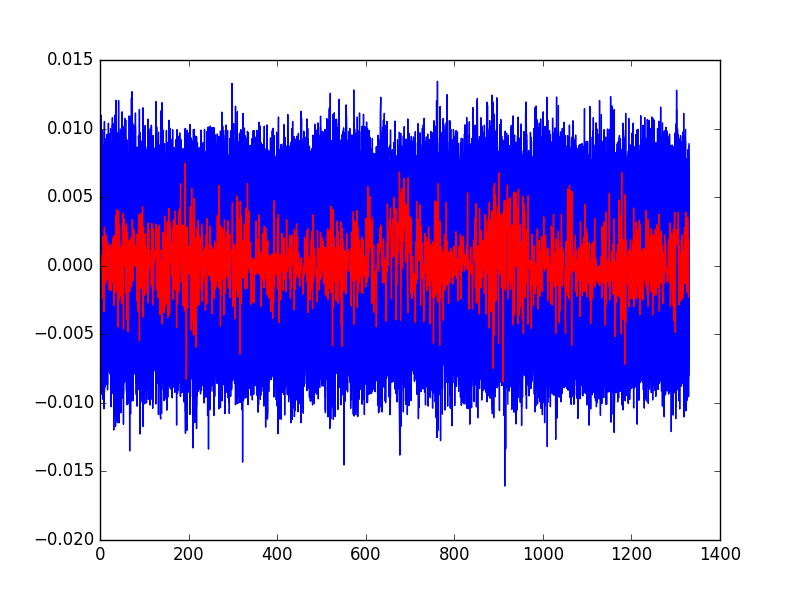
\includegraphics[scale=0.35]{figures/CPA3O_trickedZ1.png}
	\caption{Correlation coefficients obtained when targeting $S[P[i]\oplus \hat{k}] $, for every value of $\hat{k}$. Correct hypothesis plotted in red. X-axis represents all 1331 points combinations.}
	\label{fig:CPA3O_trickedZ1}
\end{figure}

\subsection{Unknown permutation, processed traces}
We now study the setting where the attacker does not know the random masks used to compute the permutation.

We preprocess the traces in order to average the leakage over the different byte indices manipulation:
\begin{itemize}
	\item for each index $i$ in $[0,15]$, we define a small window $w_i$ of $\ell$ points around the SNR peak corresponding to the manipulation of $\rmult \times S[P[Sh(i)] \oplus K[Sh(i)]]\oplus \rout$ in the characterization phase. In our experiments, the size of the window was arbitrarily fixed to $\ell=11$.
	\item for each trace in our acquisition campaign, we compute the average window $m$ such that for each time sample $j$, $m[j]=\frac{1}{16}\sum_{i=0}^{15} w_i[j]$. We then consider $m$ as our reduced averaged trace of size $\ell$.
	\item we concatenate to this trace a small window of $\ell$ points around the SNR peak corresponding to the manipulation of $\rout$.
\end{itemize}


\subsubsection{Raw Sbox output}
We target the value $Z_{\hat{k}}[i]$ for any hypothesis $k$.
The attack does not succeed using the $100.000$ traces. The correct key rank does not seem to indicate that this number of traces is close to allow a success attack.
Figure~\ref{fig:CPA3O_averagedZ1} illustrates the results using $100.000$ traces.

\begin{figure}[H]
	\centering 
	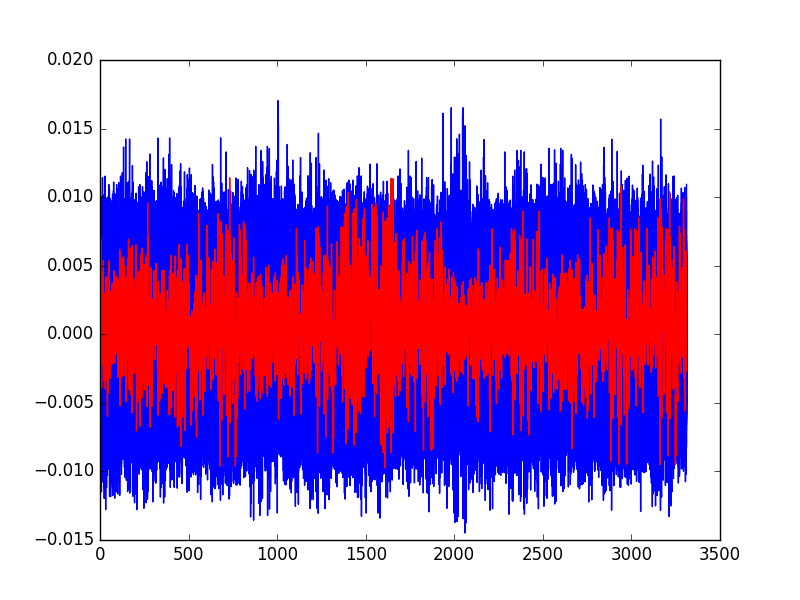
\includegraphics[scale=0.35]{figures/CPA3O_averagedZ1.png}
	\caption{Correlation coefficients obtained when targeting $S[P[i]\oplus \hat{k}] $, for every value of $\hat{k}$. Correct hypothesis plotted in red. X-axis represents all 1331 points combinations.}
	\label{fig:CPA3O_averagedZ1}
\end{figure}


\subsection{Unknown permutation, non-processed traces}
For the sake of completeness, we also perform these experiments on raw unprocessed traces. No success is obtained when targeting $Z_{\hat{k}}[i]$.
No attack is successful using $100.000$ traces.
Figure~\ref{fig:CPA3O_rawZ1} illustrates the results using $100.000$ traces.
\begin{figure}[H]
	\centering 
	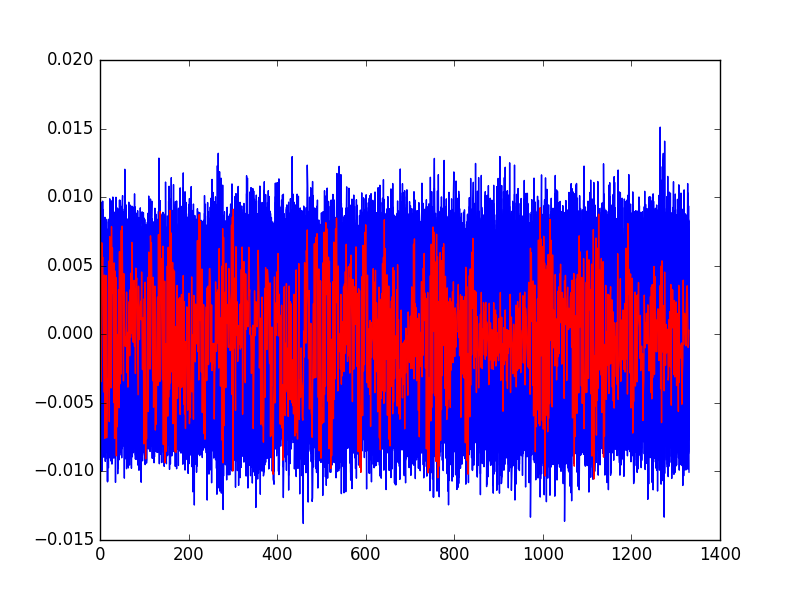
\includegraphics[scale=0.35]{figures/CPA3O_rawZ1.png}
	\caption{Correlation coefficients obtained when targeting $S[P[i]\oplus \hat{k}] $, for every value of $\hat{k}$. Correct hypothesis plotted in red. X-axis represents all 1331 points combinations.}
	\label{fig:CPA3O_rawZ1}
\end{figure}

\subsection{Summary}
No third order attack has been achieved using $100.000$ traces.
